%%%%%%%%%%%%%%%%%%%%%%%%%%%%%%%%%%%%%%%%%
% Thin Sectioned Essay
% LaTeX Template
% Version 1.0 (3/8/13)
%
% This template has been downloaded from:
% http://www.LaTeXTemplates.com
%
% Original Author:
% Nicolas Diaz (nsdiaz@uc.cl) with extensive modifications by:
% Vel (vel@latextemplates.com)
%
% License:
% CC BY-NC-SA 3.0 (http://creativecommons.org/licenses/by-nc-sa/3.0/)
%
%%%%%%%%%%%%%%%%%%%%%%%%%%%%%%%%%%%%%%%%%

%----------------------------------------------------------------------------------------
%	PACKAGES AND OTHER DOCUMENT CONFIGURATIONS
%----------------------------------------------------------------------------------------

\documentclass[a4paper, 11pt]{article} % Font size (can be 10pt, 11pt or 12pt) and paper size (remove a4paper for US letter paper)

\usepackage[protrusion=true,expansion=true]{microtype}	% Better typography
\usepackage{graphicx} 		% Required for including pictures
\usepackage{wrapfig}  		% Allows in-line images
\usepackage{hyperref}		% Allows the use of hyperlinks
\usepackage{amsmath}
\usepackage{multirow}

\usepackage{mathpazo}		% Use the Palatino font
\usepackage[T1]{fontenc} 	% Required for accented characters
\usepackage[utf8]{inputenc}     % Spanish characters
\usepackage{amsmath} 		% Allows align
\usepackage{listings}		% Allows code 
\usepackage{subfig}


\linespread{1.05} % Change line spacing here, Palatino benefits from a slight increase by default

\makeatletter
\renewcommand\@biblabel[1]{\textbf{#1.}} % Change the square brackets for each bibliography item from '[1]' to '1.'
\renewcommand{\@listI}{\itemsep=0pt} % Reduce the space between items in the itemize and enumerate environments and the bibliography

\renewcommand{\maketitle}{ % Customize the title - do not edit title and author name here, see the TITLE block below
\begin{flushright} % Right align
{\LARGE\@title} % Increase the font size of the title

\vspace{50pt} % Some vertical space between the title and author name

{\large\@author} % Author name
\\\@date % Date

\vspace{40pt} % Some vertical space between the author block and abstract
\end{flushright}
}

%----------------------------------------------------------------------------------------
%	TITLE
%----------------------------------------------------------------------------------------

\title{\textbf{Árboles de decisión}}

\author{
	\textsc{Agustín Mista}\\
	\textit{Universidad Nacional de Rosario}\\
 	\textit{Introducción a la Inteligencia Artificial}
}

\date{Rosario, 2 de Abril de 2017}

%----------------------------------------------------------------------------------------

\begin{document}

\maketitle % Print the title section

%----------------------------------------------------------------------------------------
%	ABSTRACT
%----------------------------------------------------------------------------------------

%\renewcommand{\abstractname}{Summary} % Uncomment to change the name of the abstract to something else

%\begin{abstract}
%	Cuando todo esté cocinado, voy a completar este abstract con información pertinente.
%\end{abstract}

\vspace{20pt} % Some vertical space between the abstract and first section

%----------------------------------------------------------------------------------------
%	ESSAY BODY
%----------------------------------------------------------------------------------------

\section*{Introducción}

\begin{wrapfigure}{o}{0.45\textwidth}
	\begin{center}
		\vspace{-20pt}
		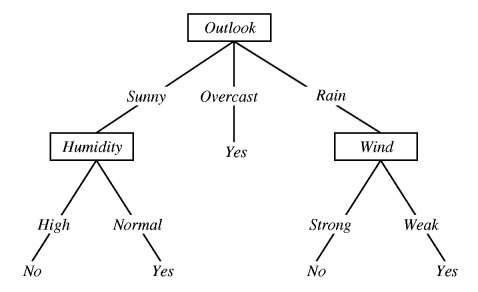
\includegraphics[width=0.4\textwidth]{play-tennis.jpg}
		\vspace{-20pt}
	\end{center}
\end{wrapfigure}

Lorem ipsum dolor sit amet, consectetur adipiscing elit. Duis id libero at
turpis varius ultrices. Proin euismod tellus ac sem porta, vel congue magna
vehicula. Nam eu viverra velit. Integer sed nulla erat. Sed interdum et urna ac
pulvinar. Sed gravida, est sit amet consectetur feugiat, enim sem molestie
lorem, a tempor orci eros ut tellus. In faucibus elit purus, feugiat viverra
nulla sodales vel. Vivamus molestie nisl enim, ac euismod purus dapibus in.
Nulla vestibulum, risus in dictum volutpat, metus nunc tristique nibh, ut
mollis diam diam commodo mi. Vestibulum ante ipsum primis in faucibus orci
luctus et ultrices posuere cubilia Curae; 

\pagebreak

%------------------------------------------------

\section*{Apartado 4}  \textit{Genere tres conjuntos de datos de entrenamiento
correspondientes al problema de las espirales anidadas de la práctica 0, uno de
longitud 150, otro de 600 y un tercero de 3000. Genere un conjunto de test de
longitud 10000. A partir de cada uno de los conjuntos de entrenamiento,
desarrolle el árbol de decisión correspondiente y grafique las predicciones
sobre el conjunto de test. Comente los resultados.}\\

Lorem ipsum dolor sit amet, consectetur adipiscing elit. Duis id libero at
turpis varius ultrices. Proin euismod tellus ac sem porta, vel congue magna
vehicula. Nam eu viverra velit. Integer sed nulla erat. Sed interdum et urna ac
pulvinar. Sed gravida, est sit amet consectetur feugiat, enim sem molestie
lorem, a tempor orci eros ut tellus. In faucibus elit purus, feugiat viverra
nulla sodales vel. Vivamus molestie nisl enim, ac euismod purus dapibus in.
Nulla vestibulum, risus in dictum volutpat, metus nunc tristique nibh, ut
mollis diam diam commodo mi. Vestibulum ante ipsum primis in faucibus orci
luctus et ultrices posuere cubilia Curae; 

\begin{figure}
  \centering
  \subfloat[][Entrenamiento]{\includegraphics[width=0.5\textwidth]{{spiral150.data}.png}}
  \subfloat[][Predicción]{\includegraphics[width=0.5\textwidth]{{spiral150.prediction}.png}}
  \caption*{\textbf{n=150}}

  \centering
  \subfloat[][Entrenamiento]{\includegraphics[width=0.5\textwidth]{{spiral600.data}.png}}
  \subfloat[][Predicción]{\includegraphics[width=0.5\textwidth]{{spiral600.prediction}.png}}
  \caption*{\textbf{n=600}}

  \centering
  \subfloat[][Entrenamiento]{\includegraphics[width=0.5\textwidth]{{spiral3000.data}.png}}
  \subfloat[][Predicción]{\includegraphics[width=0.5\textwidth]{{spiral3000.prediction}.png}}
  \caption*{\textbf{n=3000}}
\end{figure}

%------------------------------------------------

\section*{Apartado 5}  \textit{Genere tres conjuntos de datos de entrenamiento
correspondientes al problema de las espirales anidadas de la práctica 0, uno de
longitud 150, otro de 600 y un tercero de 3000. Genere un conjunto de test de
longitud 10000. A partir de cada uno de los conjuntos de entrenamiento,
desarrolle el árbol de decisión correspondiente y grafique las predicciones
sobre el conjunto de test. Comente los resultados.}\\

Lorem ipsum dolor sit amet, consectetur adipiscing elit. Duis id libero at
turpis varius ultrices. Proin euismod tellus ac sem porta, vel congue magna
vehicula. Nam eu viverra velit. Integer sed nulla erat. Sed interdum et urna ac
pulvinar. Sed gravida, est sit amet consectetur feugiat, enim sem molestie
lorem, a tempor orci eros ut tellus. In faucibus elit purus, feugiat viverra
nulla sodales vel. Vivamus molestie nisl enim, ac euismod purus dapibus in.
Nulla vestibulum, risus in dictum volutpat, metus nunc tristique nibh, ut
mollis diam diam commodo mi. Vestibulum ante ipsum primis in faucibus orci
luctus et ultrices posuere cubilia Curae; 

\begin{figure}
  \centering
  \subfloat[][Before prunning]{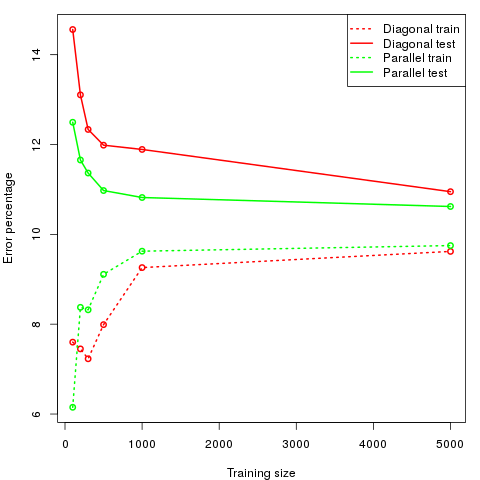
\includegraphics[width=0.5\textwidth]{sized_error_before_prunning.png}}
  \subfloat[][After prunning]{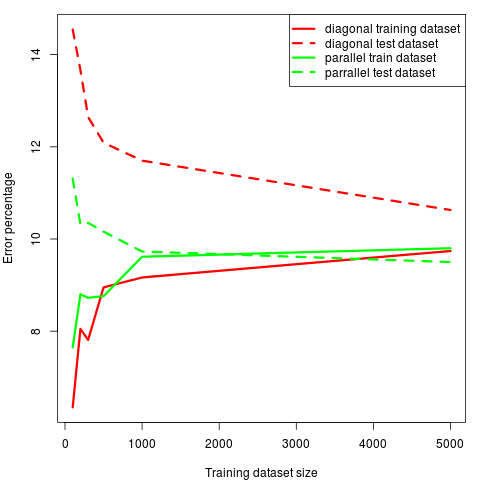
\includegraphics[width=0.5\textwidth]{sized_error_after_prunning.png}}
  \caption*{\textbf{blah blah}}

  \centering
  \subfloat[][Before prunning]{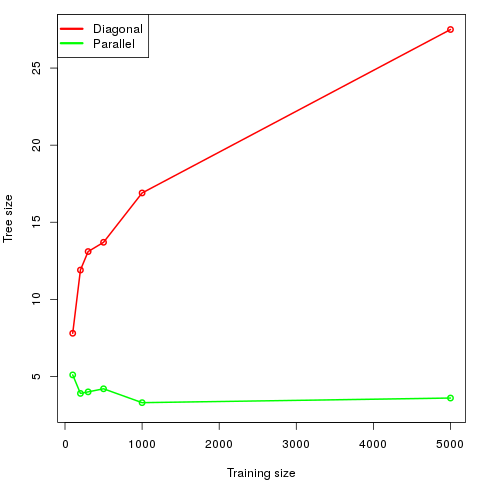
\includegraphics[width=0.5\textwidth]{sized_size_before_prunning.png}}
  \subfloat[][After prunning]{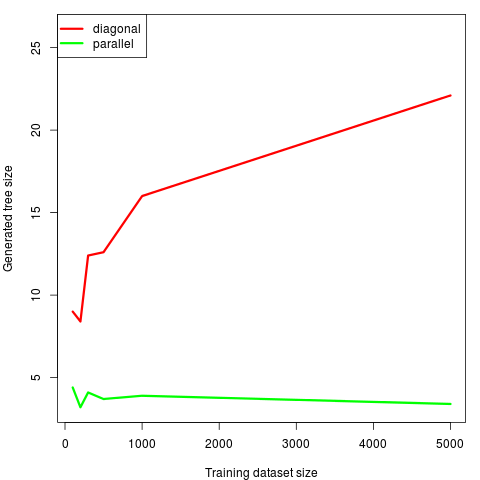
\includegraphics[width=0.5\textwidth]{sized_size_after_prunning.png}}
  \caption*{\textbf{blah blah}}

\end{figure}

%------------------------------------------------

\section*{Apartado 6}  \textit{Genere tres conjuntos de datos de entrenamiento
correspondientes al problema de las espirales anidadas de la práctica 0, uno de
longitud 150, otro de 600 y un tercero de 3000. Genere un conjunto de test de
longitud 10000. A partir de cada uno de los conjuntos de entrenamiento,
desarrolle el árbol de decisión correspondiente y grafique las predicciones
sobre el conjunto de test. Comente los resultados.}\\

Lorem ipsum dolor sit amet, consectetur adipiscing elit. Duis id libero at
turpis varius ultrices. Proin euismod tellus ac sem porta, vel congue magna
vehicula. Nam eu viverra velit. Integer sed nulla erat. Sed interdum et urna ac
pulvinar. Sed gravida, est sit amet consectetur feugiat, enim sem molestie
lorem, a tempor orci eros ut tellus. In faucibus elit purus, feugiat viverra
nulla sodales vel. Vivamus molestie nisl enim, ac euismod purus dapibus in.
Nulla vestibulum, risus in dictum volutpat, metus nunc tristique nibh, ut
mollis diam diam commodo mi. Vestibulum ante ipsum primis in faucibus orci
luctus et ultrices posuere cubilia Curae; 

\begin{figure}
  \centering
  \subfloat[][Before prunning]{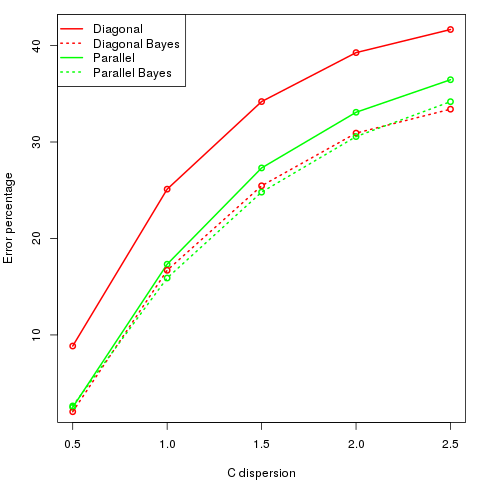
\includegraphics[width=0.5\textwidth]{noise_error_before_prunning.png}}
  \subfloat[][After prunning]{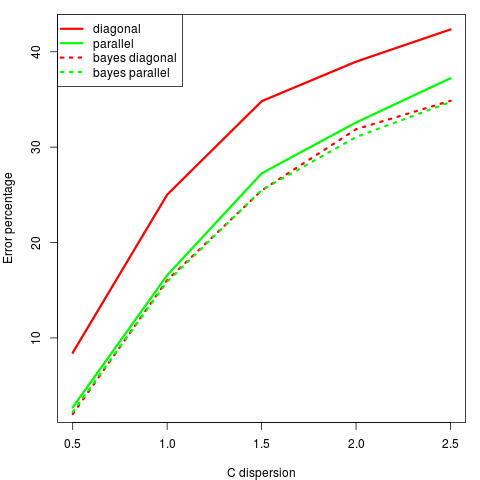
\includegraphics[width=0.5\textwidth]{noise_error_after_prunning.png}}
  \caption*{\textbf{blah blah}}

\end{figure}

%------------------------------------------------

\section*{Apartado 7}  \textit{Genere tres conjuntos de datos de entrenamiento
correspondientes al problema de las espirales anidadas de la práctica 0, uno de
longitud 150, otro de 600 y un tercero de 3000. Genere un conjunto de test de
longitud 10000. A partir de cada uno de los conjuntos de entrenamiento,
desarrolle el árbol de decisión correspondiente y grafique las predicciones
sobre el conjunto de test. Comente los resultados.}\\

Lorem ipsum dolor sit amet, consectetur adipiscing elit. Duis id libero at
turpis varius ultrices. Proin euismod tellus ac sem porta, vel congue magna
vehicula. Nam eu viverra velit. Integer sed nulla erat. Sed interdum et urna ac
pulvinar. Sed gravida, est sit amet consectetur feugiat, enim sem molestie
lorem, a tempor orci eros ut tellus. In faucibus elit purus, feugiat viverra
nulla sodales vel. Vivamus molestie nisl enim, ac euismod purus dapibus in.
Nulla vestibulum, risus in dictum volutpat, metus nunc tristique nibh, ut
mollis diam diam commodo mi. Vestibulum ante ipsum primis in faucibus orci
luctus et ultrices posuere cubilia Curae; 

\begin{figure}
  \centering
  \subfloat[][Before prunning]{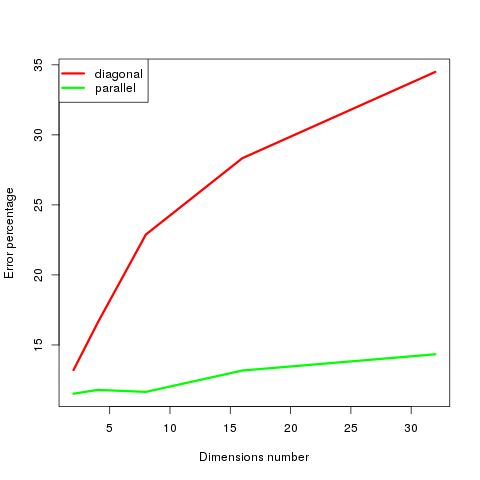
\includegraphics[width=0.5\textwidth]{dimmed_error_before_prunning.png}}
  \subfloat[][After prunning]{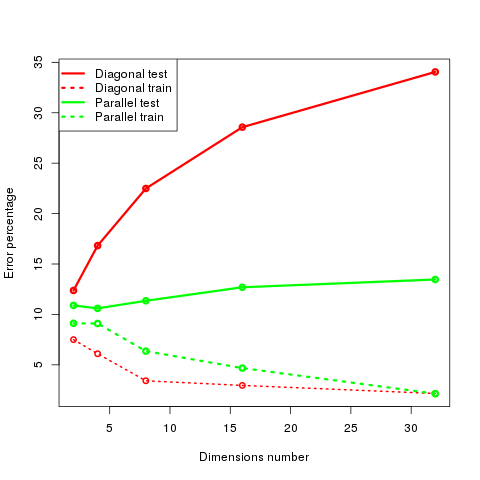
\includegraphics[width=0.5\textwidth]{dimmed_error_after_prunning.png}}
  \caption*{\textbf{blah blah}}

\end{figure}

%------------------------------------------------

\section*{Apartado 8}  \textit{Genere tres conjuntos de datos de entrenamiento
correspondientes al problema de las espirales anidadas de la práctica 0, uno de
longitud 150, otro de 600 y un tercero de 3000. Genere un conjunto de test de
longitud 10000. A partir de cada uno de los conjuntos de entrenamiento,
desarrolle el árbol de decisión correspondiente y grafique las predicciones
sobre el conjunto de test. Comente los resultados.}\\

Lorem ipsum dolor sit amet, consectetur adipiscing elit. Duis id libero at
turpis varius ultrices. Proin euismod tellus ac sem porta, vel congue magna
vehicula. Nam eu viverra velit. Integer sed nulla erat. Sed interdum et urna ac
pulvinar. Sed gravida, est sit amet consectetur feugiat, enim sem molestie
lorem, a tempor orci eros ut tellus. In faucibus elit purus, feugiat viverra
nulla sodales vel. Vivamus molestie nisl enim, ac euismod purus dapibus in.
Nulla vestibulum, risus in dictum volutpat, metus nunc tristique nibh, ut
mollis diam diam commodo mi. Vestibulum ante ipsum primis in faucibus orci
luctus et ultrices posuere cubilia Curae; 

\begin{figure}
  \centering
  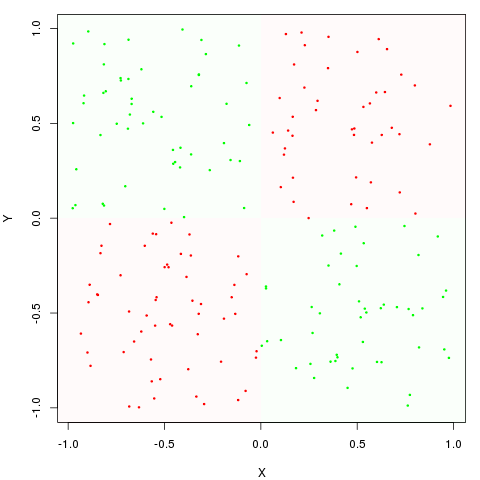
\includegraphics[width=0.7\textwidth]{xor_classes.png}
  \caption*{\textbf{blah blah}}
\end{figure}

\end{document}
